\documentclass{llncs}
\usepackage{llncsdoc}
\usepackage[hidelinks]{hyperref}
\usepackage{listings}

\usepackage{graphicx}
\setcounter{secnumdepth}{4}
\setcounter{tocdepth}{4}
\usepackage{indentfirst}
%
\begin{document}


\begin{flushleft}
\thispagestyle{empty}
\centering { \LARGE \bf Malware Meta Crawler for MASS}
\vspace{34pt}

\centering \large
 MA-INF 3309 - Malware Analysis \\
 Lab Report\\
 
   Winter Semester 2016.17\\

		 University of Bonn\\


\vspace{46pt}
\centering \large
 Ehab Qadah\\
 
 \vspace{24pt}
 
 \today\\
 \rule{\textwidth}{1pt}
\end{flushleft}

\tableofcontents

\newpage

\begin{abstract}
On a daily basis, new malware samples are discovered in. This makes the software vulnerabilities analysis one of the top concerns for organizations. The automatic identification of vulnerable software inside the organization is fundamental to avoid cyber-attacks. In this paper, we discuss two techniques to automatically monitor software vulnerabilities using open standards and public vulnerability information repositories, and alternative method to identify a vulnerable software using information obtained from social media platforms. 
\end{abstract}

\section{Introduction}

In last decade, the usage of the Internet has increased and adopted all sectors of business and industry as result of the digital
revolution. On the other hand, the wide usage of Internet creates a new opportunities for Cyber criminals to perform their malicious activities such as information theft and espionage.
Malicious Software  (malware) is any software has a harmful intention and abuse the user's computer \cite{malware_analysis_def}. Malware is a common tool to perform cyber attacks that can be in different forms such as worm, virus, Trojan and spyware \cite{worms}.
According to Symantec, in 2015, 431 million  of new malwares were discovered \cite{symantec}, which means over  one million per day. To protect the Internet's users  the malware researchers community try hardly to study these malwares, in order to build the counter measures and detect the new malware software or their malicious behavior, using different malware analysis techniques like static or dynamic analysis of malware samples \cite{malware_analysis}.

In this work, we provide malware crawler that  contentiously retrieve new malware  samples (e.g., malware domains, URLs and binary files) from different on-line sources and repositories , and submit them to MASS server to 
  build a comprehensive database of malicious software, to make the malware samples continuously available in one place, which helps the malware researchers in their studies.
  
  \par The remainder of this report is organized as follows.
  In Section~\ref{sec:sec2}, we present the related work and fundamental background . Section~\ref{sec:sec3} presents the general system overview. In Section~\ref{sec:sec4} we give the implementation details. Section~\ref{sec:sec5}
 provides the evaluation results. And finally, Section~\ref{sec:sec6} gives the overall conclusion and future work.
       
\section{Background and Related Work}
\label{sec:sec2}
- about mass 
- general overview of malware analysis 
- other people work 
- maltrieve
-Raypicker
- malware resource were used

- foundation like tool were used python + mass apiclient


In this section, we review some of the related work to our system and the required concepts that are used throughout our work.


\subsection{Malware Analysis and Storage System (MASS)}

	The Malware Analysis and Storage System (MASS) serves as a platform for  providing malware samples and analysis results \cite{mass}. All collected malware samples  and analysis results (reports) are stored in a database on the MASS server. The MASS database contains malware samples submitted by malware researchers or retrieved by the malware meta crawler component. The MASS server is connected to several analysis systems which ease the process of sample reception and analysis. In addition to that MASS provide a web interface and REST APIs to access the samples and analysis results information.
		
		The aim of MASS software is to provide the malware researchers a collaboration platform for malware analysis.

\subsection{Malware Analysis}
This section provides an overview of the malware analysis techniques (i.e., static and dynamic analysis) and the types of malware.
Bayer, Ulrich, et al. \cite{malware_analysis_def} define the malware analysis as the process of identifying and understanding the capabilities and goals of a malicious software sample. 

\subsubsection{Static Analysis:\newline }

\par The static analysis is a technique to analysis the malware sample by generating the corresponding assembly code to understand the control and data flow of the sample \cite{malware_analysis_def}. This process does not require to execute the malware sample 
\subsubsection{Dynamic Analysis:\newline } 
While the dynamic analysis approach is to study the behavior of malware sample by executing it in isolated environment \cite{malware_analysis_def}.  This process requires to run the malware executable on a certain environment and find the effects of execution on the host system. 

\subsubsection{Categories of Malware:\newline }
This section provides an overview of the different types and classes of the malware samples. The malwares are categorized based on their similar characteristic and behavior, the following are some of the malware types were observed crossed the globe \cite{malware_survey}: 
\begin{itemize}
\item Bot: 
\item Spyware:
\item virus: 
\item Trojan Horse: 
\end{itemize}
\subsection{Sources of Malware Samples } 

This section present the online sources are used in the malware meta crawler to retrieve the malware samples, while more sources can be supported in future. The following are the supported sources that contain different malware samples information:
 
\begin{itemize}
\item Malware Domain Blocklist\footnote{\url{http://www.malwaredomains.com/}}: that provides a list of malware domains that are know to used for malicious purposes.

\item Malc0de \footnote{\url{http://malc0de.com/database/}}: a database of URIs that contain  malicious executables and binaries.


\item ZeuS Tracker \footnote{\url{https://zeustracker.abuse.ch/feeds.php}}: that provides RSS feeds of IPs and domains of malicious ZeuS hosts.
\end{itemize}

\subsection{Related Systems}
\subsection{Python}

\section{System Overview}
\label{sec:sec3}
- idea +problem 
- formal algorithmic description 
- process flow diagram or any sort of charts


\subsection{Malware Meta Crawler Architecture}

\par The goal of malware meta crawler is to feed the MASS server database with new malware samples retrieved from different online sources (e.g., malwaredomains.com) which provide malicious domains or URIs that are known to be connected  with malware activities or deliver malicious payload. Furthermore, the malware metacrawler  pre-analysis the malware samples to  enrich the samples with additional related data (e.g., IP of a malware domain), also it detects the relations between the malware samples and submit it to the MASS server. Figure 1 shows the overview of the MASS project and the connection of the malware meta crawler component and analysis systems.

\begin{figure}
 
    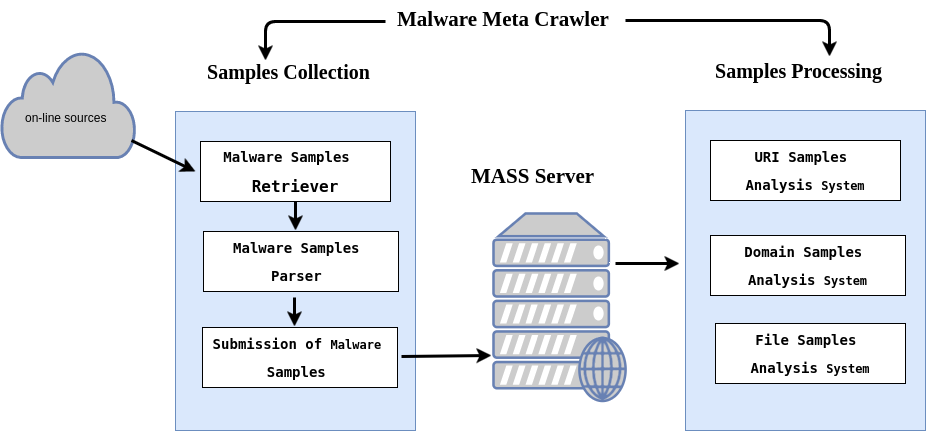
\includegraphics[width=\textwidth, height=.3\textheight]{mass1.png}
     \caption{Overview of the MASS components.}
      \label{fig:spark}
\end{figure}  

\subsection{Process Flow of Malware Meta Crawler} 

This section presents the flow of the malware meta crawler component that retrieves the 
malware samples and submit them to the MASS server. Figure 2 illustrates the internal process flow of malware meta crawler. 
 
 \begin{figure}
  \centering
     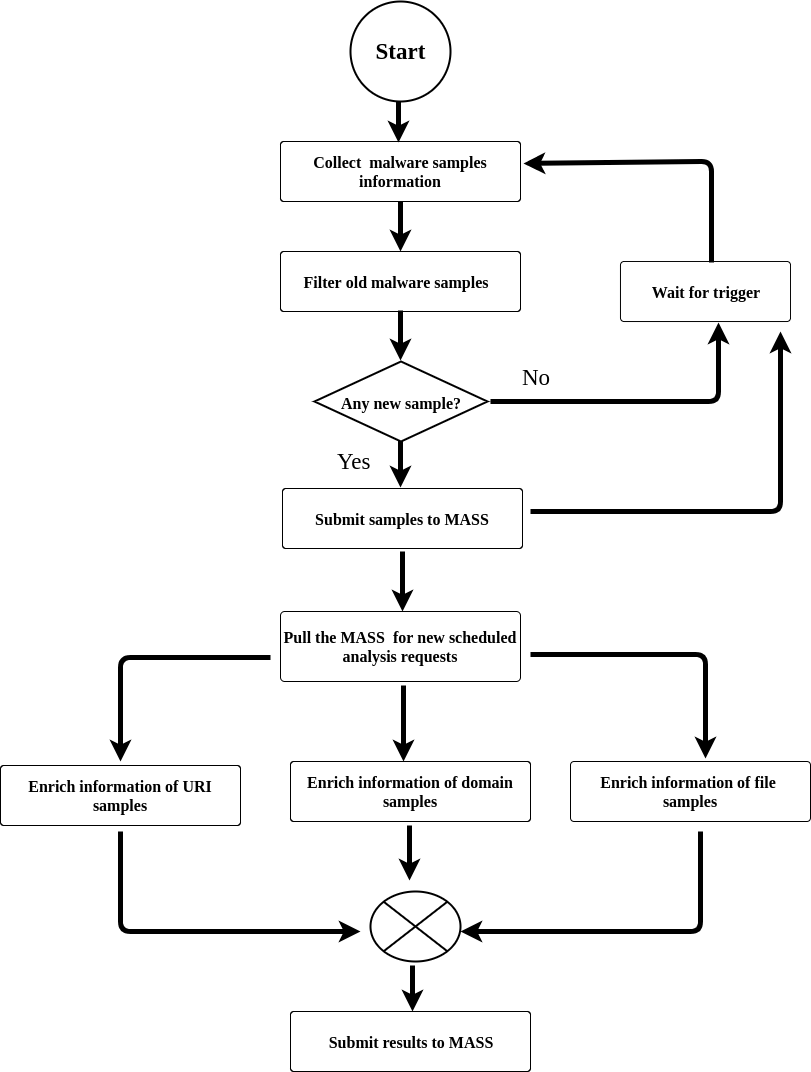
\includegraphics[]{mass2.png}
      \caption{Process flow of malware meta crawler.}
      
 \end{figure} 

\par First, the malware domains and URIs are retrieved from the mentioned sources in Section 3. Second, the retrieved list is processed to be enriched with additional information like find IP of malware domain, extract domain of malware URI and try to download the file of executable or binary URI. Third, the malware meta crawler builds the relation between the enriched malware samples such as relation between malware domain and corresponding IP, URI with malware domain and malware sample file with corresponding URI. Finlay, the malware sample and their relation with other sample are submitted to the MASS server.

\section{System Implementation}
\label{sec:sec4}
- how the idea + problem is realized + code snippet
- not code docs

\section{System Evaluation}
\label{sec:sec5}
Evaluation performance + number of samples
- state what do you like to find and how? 
- state perfomance metric like time, memory usage, etc. 
- environment setup 
- present the results 
- conclude findings

   
\section{Conclusion and Future Work}
 \label{sec:sec6}

-briefly sumup what was include/done
-state the overall achievement
-state the future work 
- measure the difference time between submission time between samples. 

\newpage
\begin{thebibliography}{[MT1]}

%

\bibitem[1]{malware_analysis_def} 
Bayer, Ulrich, et al. "Dynamic analysis of malicious code." Journal in Computer Virology 2.1 (2006): 67-77.

\bibitem[2]{worms} 
Kienzle, Darrell M., and Matthew C. Elder. "Recent worms: a survey and trends." Proceedings of the 2003 ACM workshop on Rapid malcode. ACM, 2003.

\bibitem[3]{symantec} 
Symantec. Internet Security Threat Report, Vol. 21 https://www.symantec.com/content/dam/symantec/docs/reports/istr-21-2016-en.pdf, 2016.

\bibitem[4]{malware_analysis} 
Egele, Manuel, et al. "A survey on automated dynamic malware-analysis techniques and tools." ACM Computing Surveys (CSUR) 44.2 (2012): 6.

\bibitem[5]{mass}
The Malware Analysis and Storage System(MASS). URL https://github.com/mass-project/mass\_server/blob/master/README.md.
Accessed: 2017-04-27.

\bibitem[6]{malware_survey}
Manuel Egele. A survey on automated dynamic
malware analysis techniques and tools. ACM
Computing Surveys, to appear.
%
\end{thebibliography}

\end{document}